\chapter{Statistical Modeling and Supervised Machine Learning}
\label{chap:introsml}

\begin{abstract}{Abstract} This chapter introduces the reader to the world of supervised machine learning. It starts by outlining how classical statistical techniques such as regression models can be used for prediction. It then provides an overview of frequently-used techniques from Na\"ive Bayes classifiers to neural networks.
\end{abstract}

\keywords{supervised machine learning}


\begin{objectives}
\item Understand the principles of supervised machine learning
\item Be able to run a predictive model
\item Be able to evaluate the performance of a predictive model
\end{objectives}

\newpage
\begin{feature}

 %TODO FIX
In this chapter, we use the Python package \index{statsmodels}\emph{statsmodels} for classical statistical modeling, before we move on to use a dedicated machine learning package, \index{scikit-learn}\emph{scikit-learn}. In R, we use base R for statistical modeling, \index{rsample}\emph{rsample} for splitting our dataset, \index{caret}\emph{caret} for machine learning, and \index{pROC}\emph{pROC} for determining the Receiver Operating Characteristic (ROC) curve. Note that caret requires additional packages for the actual machine learning models: \index{naivebayes}\emph{naivebayes}, \index{LiblineaR}\emph{LiblineaR}, and \index{randomforest}\emph{randomforest}. You can install them as follows (see Section~\ref{sec:installing} for more details):

\doublecodex{chapter08/chapter08install}

\noindent After installing, you need to import (activate) the packages every session:

\doublecodex{chapter08/chapter08library}

Note that in Python, we could also simply write \texttt{\small{import sklearn}} once instead of all the \texttt{\small{from sklearn import ...}} lines. But our approach saves a lot of typing later on, as we can simply write (\texttt{\small{classification\_report}}) instead of \texttt{\small{sklearn.metrics.classification\_report}}, for instance.
\end{feature}





In this chapter, we introduce the basic concepts and ideas behind
machine learning.  We will outline how machine learning relates to
traditional statistical approaches that you already might know (and as
you will see, there is a lot of overlap), present different types of
models, and discuss how to validate them.
Later in this book (Section~\ref{sec:supervised}), we will
specifically apply the knowledge you gain from this chapter to the
analysis of textual data, arguably one of the most interesting tasks
in the computational analysis of communication.

In this chapter, we focus on \emph{supervised} machine learning (SML)
-- a form of machine learning, where we aim to predict a variable
that, for at least a part of our data, is known. SML is usually applied to \textit{classification} and \textit{regression}  problems. To illustrate 
idea, imagine that you are interested in predicting  gender based
on Twitter biographies. You determine the gender for some of the
biographies yourself and hand these examples over to the computer. The
computer ``learns'' this \textit{classification} from your examples, and can then be used to predict the gender for other Twitter biographies for which you do not
know the gender.

In unsupervised machine learning (UML), in contrast, you do not have such
examples. Therefore, UML is usually applied to \textit{clustering} and \textit{associations} problems. We have discussed some  such techniques in Section~\ref{sec:clustering}, in particular cluster analysis and
principal component analysis (PCA).
Later, in Section~\ref{sec:unsupervised}, we will discuss topic modeling, an unsupervised method to extract so-called topics from textual data.


Even though both approaches can be combined (for instance, one could
first reduce the amount of data using PCA or SVD, and then predict some
outcome), they can be seen as fundamentally different,  from both
theoretical and conceptual points of view.  Unsupervised machine
learning is a bottom-up approach and corresponds to an inductive
reasoning: you do not have a hypothesis of, for instance, which topics
are present in a corpus of text; you rather let the topics emerge from
the data.  Supervised machine learning, in contrast, is a top-down
approach and can be seen as more deductive: you define \emph{a priori} which
topics to predict.


%\section{Statistical modeling and prediction}
\label{sec:prediction}
Machine learning, many people joke, is nothing else than a fancy name
for statistics.  And, in fact, there is some truth to this: If you say
``logistic regression,'' this will sound familiar to both
statisticians and machine learning practitioners.  Hence, it does not
make much sense to distinguish between statistics on the one hand and
machine learning on the other hand.

Still, there are some differences between traditional statistical
approaches that you may have learned about in your statistics classes
and the machine learning approach, even if they use some of the same
mathematical tools. One may say that  the focus is a different
one, and the objective we want to achieve may differ.

Let us illustrate this with an example.
\texttt{mediause.csv}\footnote{You can download the file from
  \url{http://cssbook.nl/d/mediause.csv}} contains a few columns from
survey data on how many days per week respondents turn to different
media types (\emph{radio}, \emph{newspaper}, \emph{tv} and \emph{internet}) in order to follow the news\footnote{For a detailed
  description of the dataset, see \citet{Trilling2013phd}.}. It also
contains their \emph{age} (in years), their \emph{gender} (coded as female = 0, male = 1), and their \emph{education} (on a 5-point scale).

A straightforward question to ask is how far the
sociodemographic characteristics of the respondents explain their
media use.  Social scientists would typically approach this question
by running a regression analysis.  Such an analysis tells us how some
independent variables $x_1, x_2 \ldots x_n$ can explain $y$.  In an
ordinary least square regression (OLS), we would estimate $y=\beta_0 +
\beta_1 x_1 + \beta_2 x_2 + \ldots + \beta_n x_n$.

In a typical social-science paper, we would then interpret the coefficients
that we estimated, and say something like: When $x_1$ increases by one unit,
$y$ increases by $\beta_1$.
We sometimes call this ``the effect of $x_1$ on $y$'' (even though, of course,
it depends on the study design weather the relationship can really be interpreted
as a causal effect).
Additionally, we might look at the explained variance $R^2$, to assess how good the model fits our data. In \refex{ols} we use this regression approach to model the relationship of \emph{age} and \emph{gender} over the number of days per week a person reads a \emph{newspaper}. We fit the linear model using the \pkg{stats} function \fn{lm} in R and the \pkg{statsmodels} (module formula.api) function \fn{ols} in Python.

\pyrex[output=py, caption=Obtaining a model through estimating an OLS regression]{chapter09/ols}

Most traditional social-scientific analyses stop after reporting and
interpreting the coefficients of \emph{age} ($\beta = 0.0676$) and \emph{gender} ($\beta = -0.0896$), as well as the total explained variance (19\%) of such a model for our dependent variable \emph{newspaper}.
But we can go a step further. Given that we have already estimated our
regression equation, why not use it to do some \textit{prediction}?

We have just estimated that

$\textrm{newspaperreading} = -0.0896 + 0.0676 \cdot \textrm{age} + 0.1767 \cdot \textrm{gender}$

By just filling in the values for a 20 year old man, or a 40 year old
woman, we can easily calculate the expected number of days such a
person reads the newspaper per week, \emph{even if no such person
  exists in the original dataset}.

We learn that

$\hat{y}_{man20} = -0.0896 + 0.0676 \cdot 20 + 1 \cdot 0.1767 = 1.4391$

$\hat{y}_{woman40} = -0.0896 + 0.0676 \cdot 40 + 0 \cdot 0.1767 = 2.6144$

This was easy to do by hand, but of course, we could do this automatically for a large and essentially unlimited number of cases.
This could be as simple as shown in \refex{olspredict}.

\pyrex[output=py, caption=Using the OLS model we estimated before to predict the dependent variable for new data where the dependent variable is unknown.]{chapter09/olspredict}

In doing so, we shift our attention from the interpretation of coefficients to the prediction of the dependent variable for new, unknown cases. We do not
care about the actual values of the coefficents, we just need them for our prediction.
In fact, in many machine learning models, we will have so many of them that
we do not even bother to report them.

As you see, this implies that we proceed in two steps: First, we use some data
to estimate our model. Second, we use that model to make predictions.

We used an OLS regression for our first example, because it is very
straightforward to interpret and most of our readers will be familiar
with it.  However, a model can take the form of \emph{any} function,
as long as it takes some characteristics (or ``features'') of the
cases (in this case, people) as input and returns a prediction.

Using such a simple OLS regression approach for prediction, as we did in our example, can come with a couple of problems, though. One problem is that in some cases, such predictions do not make much sense. For instance, even though we know that the output should be something between 0 and 7 (as that is the number of days in a week), our model will happily predict that once a man reaches the age of 105 (rare, but not impossible), he will read a newspaper on 7.185 out of 7 days. Similarly, a one year old girl will even have a negative amount of newspaper reading. A second problem relates to the models' inherent assumptions. For instance, in our example it is quite an assumption to make that the relationships between these variables are linear – we will therefore discuss multiple models that do not make such assumptions later in this chapter. And, finally, in many cases, we are actually not interested in getting an accurate prediction of a continuous number (a \textit{regression} task), but rather in predicting a category. We may want to predict whether a tweet goes viral or not, whether a user comment is likely to contain offensive language or not, whether an article is more likely to be about politics, sports, economy, or lifestyle. In machine learning terms, these tasks are known as \textit{classification}.

In the next section, we will outline key terms and concepts in machine
learning. After that, we will discuss specific models that you
can use for different use applications.

\section{Statistical Modeling and Prediction}
\label{sec:prediction}
Machine learning, many people joke, is nothing other than a fancy name
for statistics.  And, in fact, there is some truth to this: if you say
``logistic regression'', this will sound familiar to both
statisticians and machine learning practitioners.  Hence, it does not
make much sense to distinguish between statistics on the one hand and
machine learning on the other hand.
Still, there are some differences between traditional statistical
approaches that you may have learned about in your statistics classes
and the machine learning approach, even if 
some of the same
mathematical tools are used. One may say that  the focus is a different
one, and the objective we want to achieve may differ.

Let us illustrate this with an example.
\texttt{mediause.csv}\footnote{You can download the file from
  \url{http://cssbook.nl/d/mediause.csv}} contains a few columns from
survey data on how many days per week respondents turn to different
media types (\emph{radio}, \emph{newspaper}, \emph{tv} and \emph{Internet}) in order to follow the news\footnote{For a detailed
  description of the dataset, see \citet{Trilling2013phd}.}. It also
contains their \emph{age} (in years), their \emph{gender} (coded as female = 0, male = 1), and their \emph{education} (on a 5-point scale).

A straightforward question to ask is how far the
sociodemographic characteristics of the respondents explain their
media use.  Social scientists would typically approach this question
by running a regression analysis.  Such an analysis tells us how some
independent variables $x_1, x_2, \ldots, x_n$ can explain $y$.  In an
ordinary least square regression (OLS), we would estimate $y=\beta_0 +
\beta_1 x_1 + \beta_2 x_2 + \ldots + \beta_n x_n$.

In a typical social-science paper, we would then interpret the coefficients
that we estimated, and say something like: when $x_1$ increases by one unit,
$y$ increases by $\beta_1$.
We sometimes call this ``the effect of $x_1$ on $y$'' (even though, of course,
it depends on the study design whether the relationship can really be interpreted
as a causal effect).
Additionally, we might look at the explained variance $R^2$, to assess how well the model fits our data. In Example~\ref{ex:ols} we use this regression approach to model the relationship of \emph{age} and \emph{gender} over the number of days per week a person reads a \emph{newspaper}. We fit the linear model using the \index{stats}\emph{stats} function \index{lm}\texttt{lm} in R and the \index{statsmodels}\emph{statsmodels} function \index{ols}\texttt{ols} (imported from the module statsmodels.formula.api) in Python.

\pyrex[output=py, caption=Obtaining a model through estimating an OLS regression]{chapter08/ols}

Most traditional social-scientific analyses stop after reporting and
interpreting the coefficients of \emph{age} ($\beta = 0.0676$) and \emph{gender} ($\beta = -0.0896$), as well as their standard errors, confidence intervals, p-values, and the total explained variance (19\%).
But we can go a step further. Given that we have already estimated our
regression equation, why not use it to do some \textit{prediction}?

We have just estimated that

$\textrm{newspaperreading} = -0.0896 + 0.0676 \cdot \textrm{age} + 0.1767 \cdot \textrm{gender}$

By just filling in the values for a 20 year old man, or a 40 year old
woman, we can easily calculate the expected number of days such a
person reads the newspaper per week, \emph{even if no such person
  exists in the original dataset}.

We learn that

$\hat{y}_{man20} = -0.0896 + 0.0676 \cdot 20 + 1 \cdot 0.1767 = 1.4391$

$\hat{y}_{woman40} = -0.0896 + 0.0676 \cdot 40 + 0 \cdot 0.1767 = 2.6144$

This was easy to do by hand, but of course, we could do this automatically for a large and essentially unlimited number of cases.
This could be as simple as shown in Example~\ref{ex:olspredict}.

\pyrex[output=py, caption=Using the OLS model we estimated before to predict the dependent variable for new data where the dependent variable is unknown.]{chapter08/olspredict}

In doing so, we shift our attention from the interpretation of coefficients to the prediction of the dependent variable for new, unknown cases. We do not
care about the actual values of the coefficients, we just need them for our prediction.
In fact, in many machine learning models, we will have so many of them that
we do not even bother to report them.

As you see, this implies that we proceed in two steps: first, we use some data
to estimate our model. Second, we use that model to make predictions.

We used an OLS regression for our first example, because it is very
straightforward to interpret and most of our readers will be familiar
with it.  However, a model can take the form of \emph{any} function,
as long as it takes some characteristics (or ``features'') of the
cases (in this case, people) as input and returns a prediction.

Using such a simple OLS regression approach for prediction, as we did in our example, can come with a couple of problems, though. One problem is that in some cases, such predictions do not make much sense. For instance, even though we know that the output should be something between 0 and 7 (as that is the number of days in a week), our model will happily predict that once a man reaches the age of 105 (rare, but not impossible), he will read a newspaper on 7.185 out of 7 days. Similarly, a one year old girl will even have a negative amount of newspaper reading. A second problem relates to the models' inherent assumptions. For instance, in our example it is quite an assumption to make that the relationships between these variables are linear –- we will therefore discuss multiple models that do not make such assumptions later in this chapter. And, finally, in many cases, we are actually not interested in getting an accurate prediction of a continuous number (a \textit{regression} task), but rather in predicting a category. We may want to predict whether a tweet goes viral or not, whether a user comment is likely to contain offensive language or not, whether an article is more likely to be about politics, sports, economy, or lifestyle. In machine learning terms, these tasks are known as \textit{classification}.

In the next section, we will outline key terms and concepts in machine
learning. After that, we will discuss specific models that you
can use for different use applications.


%\section{Concepts and Principles}
\label{sec:principles}

%\label{sec:supervised}
The goal of Supervised Machine Learning can be summarized in one sentence:
Estimate a model based on some data, and then use the model to predict the
expected outcome for some new cases, for which we do not know the outcome yet.
This is exactly what we have done in the introductory example in Section~\ref{sec:prediction}.

But when do we need it?

In short, in any scenario where the following two preconditions are fulfilled.
First, we have a large dataset (say, $100,000$
headlines) for which we want to predict to which class they belong to (say, whether
they are clickbait or not).
Second, for a random subset of the data (say, $2,000$ of the headlines), we already
know the class.
For example because we have manually coded (``annotated'') them.

Before we start using SML, though, we first need to have
a common terminology.
At the risk of oversimplifying matters, Table~\ref{tab:mllingo} provides a rough
guideline of how some typical machine learning terms translate to statistical
terms that you may be familiar with.

\begin{table}
\caption{Some common machine learning terms explained\label{tab:mllingo}}{
  \centering
\begin{tabularx}{\textwidth}{XX}
\toprule
machine learning lingo  & statistics lingo\\ \midrule
feature                 & independent variable  \\
label                   & dependent variable  \\
labeled dataset         & dataset with both independent and dependent variables\\
to train a model        & to estimate \\
classifier (classification)  & model to predict nominal outcomes \\
to annotate             & to (manually) code (content analysis) \\
\bottomrule
\end{tabularx}}{}
\end{table}

Let us explain them more in detail by walking through a typical SML workflow.

Before we start, we need to get a \emph{labeled dataset}.
It may be given to us, or we need to create it ourselves.
For instance, often we can draw a random sample of our data and use techniques
of manual content analysis \citep[e.g.,][]{riffe2019analyzing} to
\emph{annotate} (i.e., to manually code) the data.
You can download an example for this process (annotating the topic of news
articles) from \url{http://dx.doi.org/10.6084/m9.figshare.7314896.v1} \citep{Vermeer2018}.

It is hard to give a rule of thumb for how much labelled data you need.
It depends heavily on the type of data you have (if it is a \emph{binary} or a \emph{multi-class} classification problem), and on how evenly distributed (\emph{class balance}) they are (after all, having $10,000$ annotated headlines doesn't help you if $9,990$ are no clickbait and only $10$ are).
These reservations notwithstanding, it is fair to say that typical sizes in
our field are (very roughly) speaking often in the order of $1,000$ to $10,000$
when classifying longer texts \citep[see][]{Burscher2014},
even though researchers studying less rich data sometimes annotate larger
datasets \citep[e.g., $60,000$ social media messages in][]{vermeer2019seeing}.

Once we have established that this labelled dataset is available and
have ensured that it is of good quality, we randomly split it into two
datasets: a \emph{training dataset} and a \emph{test
  dataset}.\footnote{In Section~\ref{sec:validation}, we discuss more
  advanced approaches, such as splitting into training, validation,
  and test dataset, and cross-validation.}  We will use the first one
to train our model, and the second to test how good our model
performs. Common ratios range from 50:50 to 80:20; and especially if
the size of your labelled dataset is rather limited, you may want to
have a slightly larger training dataset at the expense of a slightly
smaller test dataset.

In \refex{preparedata}, we prepare the dataset we already used in
Section~\ref{sec:prediction} for classification by creating a
dichotomous variable (the label) and splitting it into a training and
a test dataset. We use |y_train| to denote the training labels and
|X_train| to denote the feature matrix of the training dataset;
|y_test| and |X_test| is the corresponding test dataset. We set a
so-called random-state seed to make sure that the random splitting
will be the same when re-running the code. We can easily split these datasets using the \pkg{rsample} function \fn{initial\_split} in R and the \pkg{sklearn} function \fn{train\_test\_split} in Python.

\pyrex[output=py, caption=Preparing a dataset for supervised machine learning]{chapter09/preparedata}

We now can \emph{train our classifier} (i.e., estimate our model using the
training dataset contained in the objects \texttt{X\_train} and \texttt{y\_train}). This can be as straightforward as estimating a
logistic regression equation (we will discuss different classifiers in
Section~\ref{sec:nb2dnn}).  It may be that we first need to create new
independent variables, so-called features, a step known as
\emph{feature engineering}, for example by transforming existing
variables, combining them, or by converting text to numerical word
frequencies.
\refex{nb} shows how easy it is to train a classifier using the Na\"ive Bayes algorithm with packages \pkg{caret}/\pkg{naivebayes} in R and \pkg{sklearn} in Python (this approach will be better explained in Subsection~\ref{subsec:naivebayes}).

\pyrex[output=none, caption=A simple Na\"ive Bayes classifier]{chapter09/nb}

But before we can actually use this classifier to do some useful work, we need to test how capable it actually is to predict the
correct labels, given a set of features. One might think that we could
just feed it the same input data (i.e., the same features) again and
see whether the predicted labels match the actual labels of the test
dataset.  In fact, we could do that.  But this test would not be
strict enough: After all, the classifier has been trained on exactly
these data, and therefore one would expect it to perform pretty well.
In particular, it may be that the classifier is very good in
predicting its own training data, but fails at predicting other data,
because it overgeneralizes some idiosyncrasy in the data, a phenomenon
known as overfitting (see Figure ~\ref{fig:overfit}).

\begin{figure} 
\centering
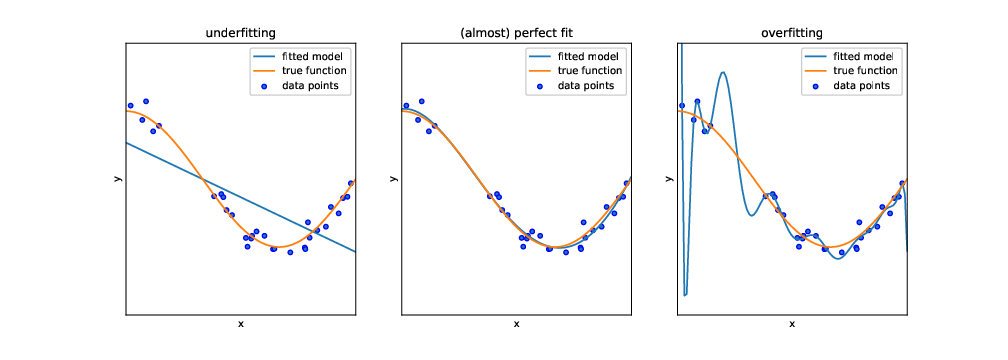
\includegraphics[width=\linewidth]{figures/ch09_overfitting}
\caption{Underfitting and overfitting. Example adapted from https://scikit-learn.org/stable/auto\_examples/model\_selection/plot\_underfitting\_overfitting.html}
\label{fig:overfit}
\end{figure}

Instead, we use the features of the \emph{test dataset} (stored in the objects  \texttt{X\_test} and \texttt{y\_test})  as input for
our classifier, and evaluate in how far the predicted labels match the
actual labels.  Remember: the classifier has at no point in time seen
the actual labels.  Therefore, we can in fact calculate how often the
prediction is right.\footnote{We assume here that the manual annotation
  is always right; an assumption that one may, of course,
  challenge. However, in the absence of any better proxy for reality,
  we assume that this manual annotation is the so-called \emph{gold
    standard} that reflects the \emph{ground truth} as closely as
  possible, and that it by definition cannot be outperformed. When creating the manual annotations, it is therefore important to safeguard their quality. In particular, one  should calculate and report some reliability measures, such as the \emph{intercoder reliability} which tests the degree of agreement between two or more annotators in order to check if our classes are well defined and the coders are doing their work correctly.}

\pyrex[output=py, caption=Calculating precision and recall]{chapter09/classificationreport}

As shown in \refex{classificationreport}, we can create a \emph{confusion matrix} (generated with \pkg{caret} function \fn{confusionMatrix} in R and \pkg{sklearn} function \fn{confusion\_matrix} in Python), and then estimate two measures: \emph{precision} and \emph{recall} (using base R calculations in R and \pkg{sklearn} function \fn{classification\_report} in Python). In a binary classification, the \emph{confusion matrix} is a useful table in which each column usually represents the number of cases in a predicted class, and each row the number of cases in the real or actual class. With this matrix (see \reffig{matrix}) we can then estimate the number of \emph{true positives} (TP) (correct prediction), \emph{false positives} (FP) (incorrect prediction), \emph{true negatives} (TN) (correct prediction) and \emph{false negatives} (FN) (incorrect prediction).


\begin{figure} 
\centering
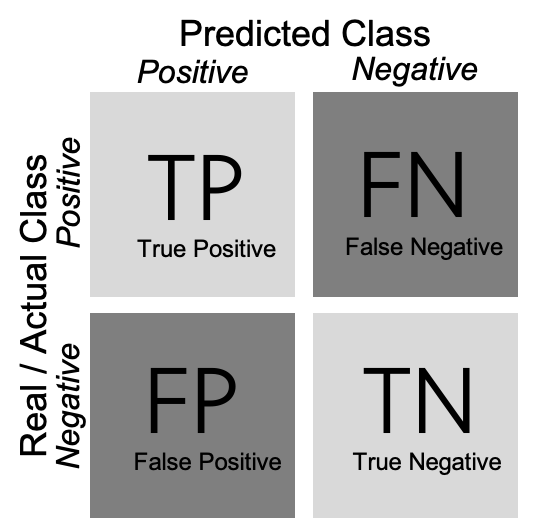
\includegraphics[width=\linewidth]{figures/ch09_matrix}
\caption{Visual representation of a confusion matrix}
\label{fig:matrix}
\end{figure}

For a better understanding of these concepts, imagine that we build a sentiment classifier, that predicts -- based on the
text of a movie review -- whether it is a positive review or a
negative review. Let us assume that the goal of training this classifier is to build an app that recommends the user only good movies. There are two things
that we want to achieve: We want to find as many positive films as possible (recall), but we also want that the selection we found
\emph{only} contains positive films (precision).

Precision is calculated as $\frac{TP}{TP+FP}$, where TP are true
positives and FP are false positives. For example, if our classifier
retrieves 200 articles that it classifies as positive films, but only
150 of them indeed are positive films, then the precision is
$\frac{150}{150+50} = \frac{150}{200} = 0.75$.

Recall is calculated as $\frac{TP}{TP+FN}$, where TP are true
positives and FN are false negatives. If we know that the classifier
from the previous paragraph missed 20 positive films, then the recall
is $\frac{150}{150+20} = \frac{150}{170}= 0.88$.

In other words: Recall measures how many of the cases we wanted to
find we actually found. Precision measures how much of what we have
found actually is correct.

Often, we have to make a trade-off between precision and recall. For
example, just retrieving \emph{every} film would give us a recall of
1.0 (after all, we didn't miss a single positive film). But on the
other hand, we retrieved all the negative films as well, so precision
will be extremely low. It can depend on the task at hand whether
precision or recall is more important. In
Section~\ref{sec:validation}, we discuss this tradeoff in detail, as well as other metrics such as \emph{accuracy}, \emph{f1-score} or the \emph{area under the curve} (AUC).

\section{Concepts and Principles}
\label{sec:principles}

%\label{sec:supervised}
The goal of Supervised Machine Learning can be summarized in one sentence:
estimate a model based on some data, and then use the model to predict the
expected outcome for some new cases, for which we do not know the outcome yet.
This is exactly what we have done in the introductory example in Section~\ref{sec:prediction}.

But when do we need it?

In short, in any scenario where the following two preconditions are fulfilled.
First, we have a large dataset (say, $100\,000$
headlines) for which we want to predict to which class they belong to (say, whether
they are clickbait or not).
Second, for a random subset of the data (say, $2000$ of the headlines), we already
know the class.
For example because we have manually coded (``annotated'') them.

Before we start using SML, though, we first need to have
a common terminology.
At the risk of oversimplifying matters, Table~\ref{tab:mllingo} provides a rough
guideline of how some typical machine learning terms translate to statistical
terms that you may be familiar with.

\begin{table}
\caption{Some common machine learning terms explained\label{tab:mllingo}}{
  \centering
\begin{tabularx}{\textwidth}{XX}
\toprule
machine learning lingo  & statistics lingo\\ \midrule
feature                 & independent variable  \\
label                   & dependent variable  \\
labeled dataset         & dataset with both independent and dependent variables\\
to train a model        & to estimate \\
classifier (classification)  & model to predict nominal outcomes \\
to annotate             & to (manually) code (content analysis) \\
\bottomrule
\end{tabularx}}{}
\end{table}

Let us explain them more in detail by walking through a typical SML workflow.

Before we start, we need to get a \emph{labeled dataset}.
It may be given to us, or we may need to create it ourselves.
For instance, often we can draw a random sample of our data and use techniques
of manual content analysis \citep[e.g.,][]{riffe2019analyzing} to
\emph{annotate} (i.e., to manually code) the data.
You can download an example for this process (annotating the topic of news
articles) from \url{http://dx.doi.org/10.6084/m9.figshare.7314896.v1} \citep{Vermeer2018}.

It is hard to give a rule of thumb for how much labeled data you need.
It depends heavily on the type of data you have (if it is a \emph{binary} or a \emph{multi-class} classification problem), and on how evenly distributed (\emph{class balance}) they are (after all, having $10\,000$ annotated headlines doesn't help you if $9990$ are not clickbait and only $10$ are).
These reservations notwithstanding, it is fair to say that typical sizes in
our field are (very roughly) speaking often in the order of $1000$ to $10\,000$
when classifying longer texts \citep[see][]{Burscher2014},
even though researchers studying less rich data sometimes annotate larger
datasets \citep[e.g., $60\,000$ social media messages in][]{vermeer2019seeing}.

Once we have established that this labeled dataset is available and
have ensured that it is of good quality, we randomly split it into two
datasets: a \emph{training dataset} and a \emph{test
  dataset}.\footnote{In Section~\ref{sec:validation}, we discuss more
  advanced approaches, such as splitting into training, validation,
  and test dataset, and cross-validation.}  We will use the first one
to train our model, and the second to test how well our model
performs. Common ratios range from 50:50 to 80:20; and especially if
the size of your labeled dataset is rather limited, you may want to
have a slightly larger training dataset at the expense of a slightly
smaller test dataset.

In Example~\ref{ex:preparedata}, we prepare the dataset we already used in
Section~\ref{sec:prediction} for classification by creating a
dichotomous variable (the label) and splitting it into a training and
a test dataset. We use |y_train| to denote the training labels and
|X_train| to denote the feature matrix of the training dataset;
|y_test| and |X_test| is the corresponding test dataset. We set a
so-called random-state seed to make sure that the random splitting
will be the same when re-running the code. We can easily split these datasets using the \index{rsample}\emph{rsample} function \index{initial\_split}\texttt{initial\_split} in R and the \index{sklearn}\emph{sklearn} function \index{train\_test\_split}\texttt{train\_test\_split} in Python.

\pyrex[output=py, caption=Preparing a dataset for supervised machine learning]{chapter08/preparedata}

We now can \emph{train our classifier} (i.e., estimate our model using the
training dataset contained in the objects \texttt{X\_train} and \texttt{y\_train}). This can be as straightforward as estimating a
logistic regression equation (we will discuss different classifiers in
Section~\ref{sec:nb2dnn}).  It may be that we first need to create new
independent variables, so-called features, a step known as
\emph{feature engineering}, for example by transforming existing
variables, combining them, or by converting text to numerical word
frequencies.
Example~\ref{ex:nb} shows how easy it is to train a classifier using the Na\"ive Bayes algorithm with packages \index{caret}\emph{caret}/\index{naivebayes}\emph{naivebayes} in R and \index{sklearn}\emph{sklearn} in Python (this approach will be better explained in Subsection~\ref{subsec:Na\"ive Bayes}).

\pyrex[output=none, caption=A simple Na\"ive Bayes classifier]{chapter08/nb}

But before we can actually use this classifier to do some useful work, we need to test how capable it  is to predict the
correct labels, given a set of features. One might think that we could
just feed it the same input data (i.e., the same features) again and
see whether the predicted labels match the actual labels of the test
dataset.  In fact, we could do that.  But this test would not be
strict enough: after all, the classifier has been trained on exactly
these data, and therefore one would expect it to perform pretty well.
In particular, it may be that the classifier is very good in
predicting its own training data, but fails at predicting other data,
because it overgeneralizes some idiosyncrasy in the data, a phenomenon
known as overfitting (see Figure ~\ref{fig:overfit}).

\begin{figure}
\centering
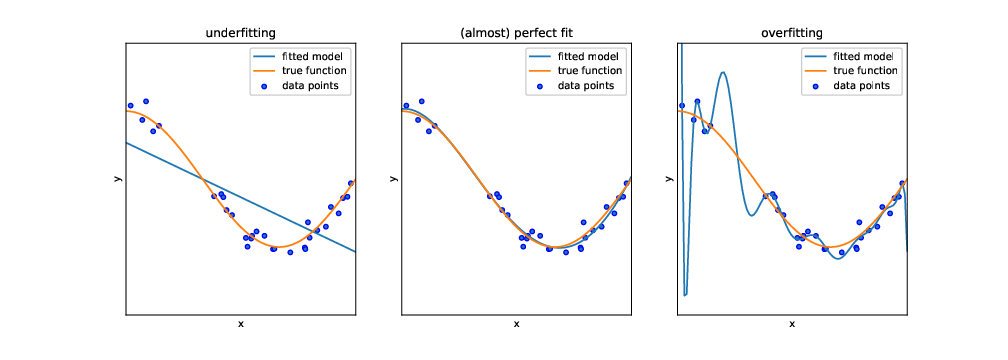
\includegraphics[width=\linewidth]{figures/ch09_overfitting}
\caption{Underfitting and overfitting. Example adapted from https://scikit-learn.org/stable/auto\_examples/model\_selection/plot\_underfitting\_overfitting.html}
\label{fig:overfit}
\end{figure}

Instead, we use the features of the \emph{test dataset} (stored in the objects  \texttt{X\_test} and \texttt{y\_test})  as input for
our classifier, and evaluate  how far the predicted labels match the
actual labels.  Remember: the classifier has at no point in time seen
the actual labels.  Therefore, we can in fact calculate how often the
prediction is right.\footnote{We assume here that the manual annotation
  is always right; an assumption that one may, of course,
  challenge. However, in the absence of any better proxy for reality,
  we assume that this manual annotation is the so-called \emph{gold
    standard} that reflects the \emph{ground truth} as closely as
  possible, and that it by definition cannot be outperformed. When creating the manual annotations, it is therefore important to safeguard their quality. In particular, one  should calculate and report some reliability measures, such as the \emph{intercoder reliability} which tests the degree of agreement between two or more annotators in order to check if our classes are well defined and the coders are doing their work correctly.}

\pyrex[output=py, caption=Calculating precision and recall]{chapter08/classificationreport}

As shown in Example~\ref{ex:classificationreport}, we can create a \emph{confusion matrix} (generated with \index{caret}\emph{caret} function \index{confusionMatrix}\texttt{confusionMatrix} in R and \index{sklearn}\emph{sklearn} function \index{confusion\_matrix}\texttt{confusion\_matrix} in Python), and then estimate two measures: \emph{precision} and \emph{recall} (using base R calculations in R and \index{sklearn}\emph{sklearn} function \index{classification\_report}\texttt{classification\_report} in Python). In a binary classification, the \emph{confusion matrix} is a useful table in which each column usually represents the number of cases in a predicted class, and each row the number of cases in the real or actual class. With this matrix (see Figure~\ref{fig:matrix}) we can then estimate the number of \emph{true positives} (TP) (correct prediction), \emph{false positives} (FP) (incorrect prediction), \emph{true negatives} (TN) (correct prediction) and \emph{false negatives} (FN) (incorrect prediction).


\begin{figure}
\centering
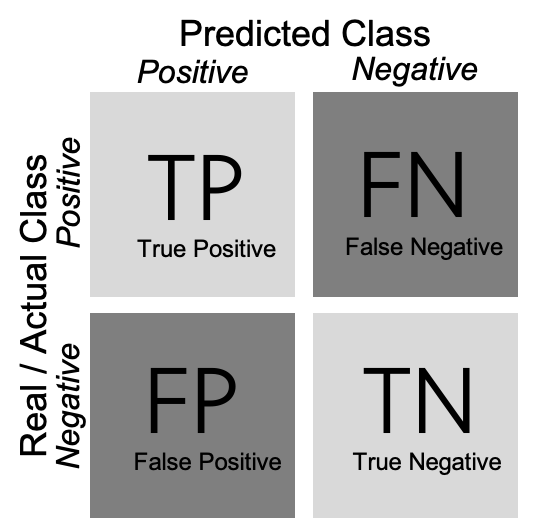
\includegraphics[width=\linewidth]{figures/ch09_matrix}
\caption{Visual representation of a confusion matrix.}
\label{fig:matrix}
\end{figure}

For a better understanding of these concepts, imagine that we build a sentiment classifier, that predicts -- based on the
text of a movie review -- whether it is a positive review or a
negative review. Let us assume that the goal of training this classifier is to build an app that recommends only good movies to the user. There are two things
that we want to achieve: we want to find as many positive films as possible (recall), but we also want that the selection we found
\emph{only} contains positive films (precision).

Precision is calculated as $\frac{\rm{TP}}{\rm{TP}+\rm{FP}}$, where TP are true
positives and FP are false positives. For example, if our classifier
retrieves 200 articles that it classifies as positive films, but only
150 of them indeed are positive films, then the precision is
$\frac{150}{150+50} = \frac{150}{200} = 0.75$.

Recall is calculated as $\frac{\rm{TP}}{\rm{TP}+\rm{FN}}$, where TP are true
positives and FN are false negatives. If we know that the classifier
from the previous paragraph missed 20 positive films, then the recall
is $\frac{150}{150+20} = \frac{150}{170}= 0.88$.

In other words: recall measures how many of the cases we wanted to
find we actually found. Precision measures how much of what we have
found actually is correct.

Often, we have to make a trade-off between precision and recall. For
example, just retrieving \emph{every} film would give us a recall of
1.0 (after all, we didn't miss a single positive film). But on the
other hand, we retrieved all the negative films as well, so precision
will be extremely low. It can depend on the task at hand whether
precision or recall is more important. In
Section~\ref{sec:validation}, we discuss this trade-off in detail, as well as other metrics such as \emph{accuracy}, \emph{$F_1$-score} or the \emph{area under the curve} (AUC).

%\section{From Na\"{i}ve Bayes to Deep Neural Networks}
\label{sec:nb2dnn}

\section{Classical Machine Learning: From Na\"{i}ve Bayes to Neural Networks}
\label{sec:nb2dnn}
To do supervised machine learning, we can use several models, all of
which have different advantages and disadvantages, and are more useful
for some use cases than for others.
We limit ourselves to the most common ones in this chapter. The
website of scikit-learn (\url{http://www.scikit-learn.org}) gives a
good overview of more alternatives.

\subsection{Na\"ive Bayes}
\label{subsec:Na\"ive Bayes}

The Na\"ive Bayes classifier is a very simple classifier that is often
used as a ``baseline''. Before estimating more complicated and
resource-intensive models, it is a good idea to estimate a simpler
model first, to assess how much better the other model actually
is. Sometimes, the simple model might even be just fine.

The Na\"ive Bayes classifier allows you to predict a binary outcome,
such as: ``Is this message spam or not?'', ``Is this article about
politics or not?'', ``Will this go viral or not?''.  It, in fact, also
allows you to do the same with more than one category, and both the
Python and the R implementation will happily let you train a Na\"ive
Bayes classifier on nominal data, such as whether an article is about
politics, sports, the economy, or something different.

For the sake of simplicity, we will discuss a binary example, though.

As its name suggests, a Na\"ive Bayes classifier is based on Bayes'
theorem, and it is ``na\"ive''.  It may sound a bit weird to call a
model ``na\"ive'', but what it actually means is not so much that it
is stupid, but that it makes very far-reaching assumptions about the
data (hence, it is na\"ive). Specifically, it assumes that all
features are independent from each other.  Of course, that is hardly
ever the case -- for instance, in a survey data set, while age and
gender indeed are generally independent from each other, this is not the case for education, political interest,
media use, and so on.  And in textual data, whether a word $W_1$ is used
is not independent from the use of word $W_2$ -- after all, both are not
randomly drawn from a dictionary, but depend on the topic of the text
(and other things).  Astonishingly, even though these assumptions are
regularly violated, the Na\"ive Bayes classifier works reasonably well
in practice.

The Bayes part of the Na\"ive Bayes classifier comes from the fact
that it uses Bayes' formula, $$ P(\rm{A} \mid \rm{B}) = \frac{P(\rm{B} \mid \rm{A}) \cdot P(\rm{A})}{P(\rm {B})} $$.

As a short refresher: The $P(\rm{A} \mid \rm{B})$ can be read as: the
probability of A, given B. Or: the probability of A if B is the
case/present/true.  Applied to our problem, this means that we are
interested in estimating the probability of an item having a label,
given a set of features:
$$ P(\rm{label} \mid \rm{features}) = \frac{P(\rm{features} \mid \rm{label}) \cdot P(\rm{label})}{P(\rm{features})} $$.

P(label) can be easily calculated: it's just the fraction of all
cases with the label we are interested in.  Because we assume that our
features are independent (remember, the ``na\"ive'' part), we can
calculate P(features) and P(features$\mid$label) by just
multiplying the probabilities of each individual feature.  Let's
assume we have three features, $x_1, x_2, x_3$.  We now simply
calculate the percentage of \emph{all} cases that contain these
features, ${P}(x_1), {P}(x_2)$ and ${P}(x_3)$.  Then we do the same for the
conditional probabilities and calculate the percentage of cases
\emph{with our label} that contain these features, ${P}(x_1\mid \rm{label}),
{P}(x_2\mid \rm{label})$ and ${P}(x_3\mid \rm{label})$.

If we fill this in our formula, we get:


$$ P(\rm{label} \mid \rm{features}) = \frac{P(x_1 \mid label) \cdot P(x_2 \mid \rm{label})\ \cdot P(x_3 \mid label) \cdot P(label)}{P(x_1) \cdot P(x_2) \cdot P(x_3)}$$.

Remember that all we need to do to calculate this formula is: (1)
count how many cases we have in total; (2) count how many cases
have our label; (3) count how many cases in (1) have feature $x$;
(4) count  how many cases in (2) have feature $x$.  As you can
imagine, doing this does not take much time to do, which is what makes the
Na\"ive Bayes classifier such a fast and efficient choice.  This may
in particular be true if you have a lot of features (i.e.,
high-dimensional data).

Counting whether a feature is present or not, of course, is only
possible for binary data. We could for example simply check whether a
given word is present in a text or not.  But what if our features are
continuous data, such as the number of times the word is present?  We
could dichotomize it, but that would discard information.  So, what
we do instead, is that we estimate P$(x_i)$ using a distribution, for
example a Gaussian, Bernoulli, or multinomial distribution. The core
idea, though, stays the same.

Our examples in Section~\ref{sec:principles} illustrate how to train a Na\"ive Bayes classifier.
We first create the labels (whether someone uses online news at all or
not), split our data into a training and a test dataset (here, we use
80\% for training and 20\% for testing) (Example~\ref{ex:preparedata}), then
fit (train) a classifier (Example~\ref{ex:nb}), before we assess how well it
predicts our training data (Example~\ref{ex:classificationreport}).

In Section~\ref{sec:validation}, we discuss in more detail how to
evaluate different classifiers, but let's have a sneak preview at the most used
measures of how well our classifier performs.
The confusion matrix from Example~\ref{ex:classificationreport} tells us how many non-users were indeed
classified as non-users (59), and how many (wrongly) as users
(102).\footnote{These are the values from the Python example, the R
  example slightly differs, amongst other things due to different
  sampling.} That doesn't look very good; but on the other hand, 210
of the true users were correctly classified as such, and only 42 were
not.

More formally, we can express this using precision and recall. When we
are interested in finding true users, we get a precision of $\frac{212}{212+106} = 0.67$
 and a recall of $\frac{212}{212+40} = 0.84$.
However, if we want to know how good we are in identifying those who
do \emph{not} use online news, we do -- as we saw in the confusion
matrix -- considerably worse: precision and recall are 0.58 and 0.34,
respectively.



\subsection{Regression}
\label{subsec:regression}

Regression analysis does not make as strong an assumption about the
independence of features as the Na\"ive Bayes classifier does.  Sure,
we have been warned about the dangers of multicollinearity in
statistics classes, but correlation between features (for which
multicollinearity is a fancy term) affects the coefficients and their
$p$ values, but not the predictions of the model as a whole.   To put
it differently, in regression models, we do not estimate the
probability of a label given a feature, independent of all the other
features, but are able to ``control for'' their influence.  In theory,
this should make our models better, and also in practice, this
regularly is the case. However, ultimately, it is an empirical
question which model performs best.

While we started this chapter with an example of an OLS regression to
estimate a continuous outcome (well, by approximation, as for ``days
per week'' not all values make sense), we will now use a regression
approach to predict nominal outcomes, just as in the Na\"ive Bayes
example.  The type of regression analysis to use for this is called
\emph{logistic regression}.

In a normal OLS regression, we estimate

$$y = \beta_o + \beta_1 x_1 + \beta_2 x_2 + \ldots + \beta_n x_n$$

But this gives us a continuous outcome, which we do not want. In a
logistic regression, we therefore use the sigmoid function to map this
continuous outcome to a value between 0 and 1. The sigmoid function is
defined as $sigmoid(x) = \frac{1}{1 + e^{-x}}$ and depicted in
Figure~\ref{fig:sigmoid}.

\begin{figure}
  \centering
\begin{tikzpicture}
    \begin{axis}%
    [
        grid=major,
        xmin=-6,
        xmax=6,
        axis x line=bottom,
        ytick={0,.5,1},
        ymax=1,
        axis y line=middle,
    ]
        \addplot%
        [
            black,%
            mark=none,
            samples=100,
            domain=-6:6,
        ]
        (x,{1/(1+exp(-x))});
    \end{axis}
\end{tikzpicture}
\caption{\label{fig:sigmoid} The sigmoid function.}
\end{figure}


Combining these formulas gives us:

$$P = \frac{1}{1 + e^{-(\beta_o + \beta_1 x_1 + \beta_2 x_2 = \ldots + \beta_n x_n)}} $$


Wait, you might say. Isn't $P$ still continuous, even though it is now
bounded between 0 and 1? Yes, it is.  Therefore, after having
estimated the model, we use a threshold value (typically, 0.5, but we will discuss in Section~\ref{sec:balance} how to select different ones) to
predict the label. If $P>0.5$, we predict that the case is spam/about
politics/will go viral, if not, we predict it's not.
A nice side effect of this is that we still can use the probabilities
in case we are interested in them, for example to figure out for which
cases we are more sure in our prediction.

Just as with the Na\"ive Bayes classifier, also for logistic
regression classifiers, Python and R will happily allow us to estimate
models with multiple nominal outcomes instead of a binary outcome. In Example~\ref{ex:logreg} we fit the logistic regression using the \index{caret}\emph{caret} method \index{logreg}\texttt{logreg} in R and the \index{sklearn}\emph{sklearn} (module linear\_model) function \index{LogisticRegression}\texttt{LogisticRegression} in Python.

And, of course, you actually can do OLS regression (or more advanced
regression models) if you want to estimate a continuous outcome.


\pyrex[output=none, caption=A simple logistic regression classifier]{chapter08/logreg}



\subsection{Support Vector Machines}
Support Vector Machines (SVM) are another very popular and versatile
approach to supervised machine learning.  In fact, they are quite
similar to logistic regression, but try to optimize a different
function. In technical terms, SVM minimizes \emph{hinge loss} instead
of logistic loss.

What does that mean to us? When estimating logistic regressions, we
are interested in estimating probabilities, while when training a
SVM, we are interested in finding a plane (more
specifically, a hyperplane) that best separates the data points of the
two classes (e.g., spam versus non-spam messages) that we want to
distinguish.  This also means that a SVM does not give you
probabilities associated with your prediction, but just the label.
But usually, that's all that you want anyway.

Without going into mathematical detail here (for that, a good source
would be \citet{kelleher2015fundamentals}), we can say that finding the
widest separating margin that we can achieve constructing a plane in a
graphical space (SVM) versus optimizing a log-likelihood function
(logistic regression) results in a model that is less sensitive to
outliers, and tends to be more balanced.

There are a lot of graphical visualizations available, for example in
the notebooks supplementing \cite{vanderplas2016python}
(\url{https://jakevdp.github.io/PythonDataScienceHandbook/05.07-support-vector-machines.html}).
For now, it may suffice to imagine the two-dimensional case: we
construct a line that separates two groups of dots \emph{with the
  broadest possible margin}. The dots that the margin of this line
just touches are called the ``support vectors'', hence the name.

You could imagine that sometimes we may want to be a bit lenient
about the margins. If we have thousands of data points, then maybe it
is okay if one or two of these data points are, in fact, within the
margin of the separating line (or hyperplane). We can control this with
a parameter called $C$: For very high values, this is not allowed, but
the lower the value, the ``softer'' the margin is.  In
Section~\ref{sec:crossvalidation}, we will show an approach to find
the optimal value.

A big advantage of SVMs is that they can be extended to non-linear
separable classes. Using a so-called kernel function or \emph{kernel trick}, we can transform
our data so that the dataset becomes linearly separable. Choices
include but are not limited to multinomial kernels, the radial basis
function (RBF), or Gaussian kernels. If we, for example, have  two
concentric rings of data points (like a donut), then we cannot find a
straight line separating them. But a RBF kernel can transfer them into
a linearly separable space. The aforementioned online visualizations
can be very instructive here.

Example~\ref{ex:svm} shows how we implement standard SVM to our data using the \index{caret}\emph{caret} method \index{svmLinear3}\texttt{svmLinear3} in R and the \index{sklearn}\emph{sklearn} (module svm) function \index{SVC}\texttt{SVC} in Python. You can see in the code that feature data is standardized or normalized (with $m = 0$ and $\rm{std} = 1$) before model training in order to have all the features measured at the same scale, as required by SMV.

\pyrex[output=none, caption=A simple Support Vector Machine classifier]{chapter08/svm}



\subsection{Decision Trees and Random Forests}
\label{subsec:randomforest}
In the models we have discussed so far, we were essentially  modeling linear
relationships. If the value of a feature is twice as high, its
influence on the outcome will be twice as high as well.  Sure, we can
(and do, as in the case of the sigmoid function or the SVM kernel trick) apply some
transformations, but we have not really considered yet how we can
model situations in which, for instance, we care about whether the
value of a feature is above (or below) a specific threshold.  For
instance, if we have a set of social media messages and want to model
the medium from which they most likely come, then its length is very
important information. If it is longer than 280 characters (or,
historically, 140), then we can be \emph{very} sure it is not from
Twitter, even though the reverse is not necessarily true. But it does
not matter at all whether it is 290 or $10\,000$ characters long.

Entering this variable into a logistic regression, thus, would not be
a smart idea.  We could, of course, dichotomize it, but that would
only partly solve the problem, as its effect can still be overridden by other variables.  In this example, we \emph{know} how to
dichotomize it based on our prior knowledge about the number of
characters in a tweet, but this does not necessarily need to be the
case; it might be something we need to estimate.

A step-wise decision, in which we first check one feature (the
length), before checking another feature, can be modeled as a decision
tree.  Figure~\ref{fig:decisiontree} depicts a (hypothetical) decision
tree with three \textit{leaves}.

\begin{figure}
  \centering
\begin{tikzpicture}[
    node/.style={%
      draw,
      rectangle,
    },
  ]

    \node [node] (A) {Number of characters};
    \path (A) ++(-135:30mm) node [node] (B) {FB-post};
    \path (A) ++(-45:30mm) node [node] (C) {Uses hashtag?};
    \path (C) ++(-135:30mm) node [node] (D) {Tweet};
    \path (C) ++(-45:30mm) node [node] (E) {FB-post};

    \draw (A) -- (B) node [left,pos=0.25] {$>280$}(A);
    \draw (A) -- (C) node [right,pos=0.25] {$<280$}(A);
    \draw (C) -- (D) node [left,pos=0.25] {yes}(A);
    \draw (C) -- (E) node [right,pos=0.25] {no}(A);
\end{tikzpicture}
  \caption{\label{fig:decisiontree}A simple decision tree.}
\end{figure}

Faced with the challenge to predict whether a social media message is
a tweet or a Facebook post, we could predict 'Facebook post' if its
length is greater than 280 characters. If not, we check whether it
includes hashtags, and if so, we predict 'tweet', otherwise, 'Facebook
post'.
Of course, this simplistic model will be wrong at some times, because
not all tweets have hashtags, and some Facebook posts actually do
include hashtags.

While we constructed this hypothetical decision tree by hand, usually,
we are more interested in learning such non-linear relationships from
the data.  This means that we do not have to determine the cutoff
point ourselves, but also that we do not determine the order in which
we check multiple variables by hand.

Decision trees have two nice properties. First, they are very easy to
explain.  In fact, a figure like Figure~\ref{fig:decisiontree} is
understandable for non-experts, which can be important in scenarios
where for accountability reasons, the decision of a classifier must be
as transparent as possible.  Second, they allow us to approximate
almost all non-linear relationships (be it not necessarily very
accurately).

However, this comes at large costs.  Formulating a model as a series
of yes/no questions, as you can imagine, inherently loses a lot of
nuance. More importantly, in such a tree, you cannot ``move up''
again. In other words, if you make a wrong decision early on in the
tree (i.e., close to its root node), you cannot correct it later.
This rigidity makes decision trees also prone to overfitting: they may
fit the training data very well, but may not generalize well enough to
slightly different (test) data.

Because of these drawbacks, decision trees are seldom used in
real-life classification tasks.  Instead, one uses an \emph{ensemble} model: so-called random forests.  Drawing random samples from the data, we estimate multiple
decision trees -- hence, a forest.  To arrive at a final prediction,
we can then  let the trees ``vote'' on which label we should
predict. This procedure is called ``majority voting'', but there are
also other methods available. For example, \index{scikit-learn}\emph{scikit-learn} in Python  by default uses a method called \index{probabilistic prediction}\texttt{probabilistic prediction}, which takes into
account probability values instead of simple votes.

In Example~\ref{ex:randomforest} we create a random forest classifier with 100 trees using the \index{caret}\emph{caret} method \index{rf}\texttt{rf} in R and the \index{sklearn}\emph{sklearn} (module ensamble) function \index{RandomForestClassifier}\texttt{RandomForestClassifier} in Python.

\pyrex[output=none, caption=A simple Random Forest classifier]{chapter08/randomforest}

Because random forests alleviate the problems of decision trees, but
keep the advantage of being able to model non-linear relationships,
they are frequently used when we expect such relationships (or have no
idea about what  the relationship looks like).  Also, random forests may
be a good choice if you have very different types of features (some
nominal, some continuous, etc.) in your model. The same holds true if
you have a lot (really a lot) of features: methods like SVM would require
constructing large matrices in memory, which random forests do not.
But if the relationships between your features and your labels are
actually (approximately) linear, then you are probably better off with
one of the other models we discussed.


\subsection{Neural Networks} \label{sec:neural}

The machine learning algorithms that we will discuss here are neural networks.
Inspired by the neurons in the brains of humans (and  other animals),
neural networks consist of connections between neurons that are activated if the
total input is above a certain threshold.

Figure~\ref{fig:perceptron} shows the simplest type of neural network, sometimes called a \index{perceptron}\emph{perceptron}.
This neural network consists only of a series of input neurons (representing the features or independent variables)
which are directly connected with the output neuron or neurons (representing the output class(es)).
Each of the connections between neurons has a weight, which can be positive or negative.
For each output neuron, the weighted sum of inputs is calculated and a function is applied to determine the result.
An example output function is the sigmoid function (Figure~\ref{fig:sigmoid}) which transforms the output to a value between zero and one,
in which case the resulting model is essentially a form of logistic regression.

\begin{figure}
  \centering
 \begin{neuralnetwork}[height=4]
        \newcommand{\x}[2]{$x_#2$}
        \newcommand{\y}[2]{$\hat{y}_#2$}
        \inputlayer[count=3, bias=true, title=Input\\layer, text=\x]
        \outputlayer[count=1, title=Output\\layer, text=\y] \linklayers
 \end{neuralnetwork}
\caption{Schematic representation of a typical classical machine learning model. \label{fig:perceptron}}
\end{figure}

If we consider a neural network for sentiment analysis of tweets,
the input neurons could be the frequencies of words such as ``great'' or ``terrible'',
and we would assume that the weight of the first would be positive while the second would be negative.
Such a network cannot take combinations into account, however:
the result of ``not great'' will simply be the addition of the results of ``not'' and ``great''.

To overcome this limitation, it is possible to add a \index{hidden layer}\emph{hidden layer} of latent variables
between the input and output layer, such as shown in Figure~\ref{fig:hiddenlayers}.
This allows for combinations of neurons, with for example both ``not'' and 	``great'' loading onto a hidden neuron,
which can then override the direct effect of ``great''.
An algorithm called \index{backpropagation}\emph{backpropagation} can be used to iteratively approximate the optimal values for the model.
This algorithm starts from a random state and optimizes the second layer while keeping the first constant,
then optimizing the first layer, and repeating until it converges.

Although such hidden layers, which can easily contain thousands of neurons, are hard to interpret substantively,
they can substantially improve the performance of the model.
In fact, the Universal Approximation theorem states that every decision function can be approximated to infinite precision
with a single (but possibly very large) hidden layer \citet{goldberg2017}.
Of course, since training data is always limited there is a practical limit to how deep or wide the network can be,
but this shows the big difference that a hidden layer can make in the range of regularities that can be ``captured'' in the model.

\begin{figure}
  \centering
 \begin{neuralnetwork}[height=5]
        \newcommand{\x}[2]{$x_#2$}
        \newcommand{\y}[2]{$\hat{y}_#2$}
        \newcommand{\hfirst}[2]{\small $h^{(1)}_#2$}
        \newcommand{\hsecond}[2]{\small $h^{(2)}_#2$}
        \inputlayer[count=3, bias=true, title=Input\\layer, text=\x]
        \hiddenlayer[count=5, bias=false, title=Hidden\\layer 1, text=\hfirst] \linklayers
        \hiddenlayer[count=3, bias=false, title=Hidden\\layer 2, text=\hsecond] \linklayers
        \outputlayer[count=1, title=Output\\layer, text=\y] \linklayers
 \end{neuralnetwork}
\caption{A neural network. \label{fig:hiddenlayers}}
\end{figure}

%Neural networks with and without hidden layers can be easily trained in either Python or R,
%as shown in Example~\ref{ex:neuralnetwork}.
%% TODO: insert example



%\section{Deep Learning}
\label{sec:deeplearning}

In \refsec{neural}, we introduced neural networks with hidden layers and the backpropagation algorithm to fit them,
both of which date back to at least the 1970's.
In the past decade, however, the Artificial Intelligence community is transformed by the introduction of \concept{deep learning},
where deep refers to a large amount of hidden layers between the input and output layers.
Many of the recent advances in AI, from self-driving cars to automatic translation and voice assistants,
are made possible by the application of deep learning techniques to the enormous amounts of digital data now becoming available. 

An extensive treatment of Deep Learning is beyond the scope of this book (we recommend \cite{geron2019hands} instead).
However, in this section we will give you a brief introduction that should help you understand deep learning at a conceptual level,
and in \refchap{dtm} and \refchap{image} we will explain how these techniques can be applied to text analysis and visual analysis, respectively. 

In principle, there is no clear demarcation between a `classical' neural network with hidden layers and a `deep' neural network.
There are three properties, however, that distinguish deep learning and explain why it is so succesful: scale, structure, and feature learning.

\paragraph{Scale} First, and perhaps most importantly, deep learning models are many orders of magnitude larger and more complex than the models
trained in earlier decades.
This has been made possible by the confluence of unprecedented amounts of digital training data and increased computer processing power.
Party, this is enabled by the use of graphical processing units (GPUs), hardware designed for rendering the 3D worlds used in games,
but that can also be used very efficiently for the computations needed to train neural networks (and mine bitcoins, but that's another story).

\paragraph{Structure} Most classical neural networks have only `fully connected' hidden layers with forward propagation,
meaning that each neuron in one layer is connected to each neuron in the next layer.
In deep learning, many specific architectures (some of which will be discussed below) are used to process information in certain ways,
limiting the number of parameters that need to be estimated.

\paragraph{Feature Learning}
In all models described so far with the exception of neural networks with hidden layers,
there was a direct relationship between the input features and the output class.
This meant that it is important to make sure that the required information the model needs to distinguish the classes
is directly encoded in the input features.
In the example used earlier, if `not' and `good' are separate features, a single-layer network (or a Na\"ive Bayes model)
cannot learn that these words together have a different meaning than the addition of their separate meanings.
However, similar to regression analysis, where you can create an interaction term or squared term to model a non-linear relationship,
the researcher can create input features for e.g. word pairs, for example including bigrams (word pars) such as `not\_good`.
In fact, engineering the right features was the main way in which a researcher could improve model performance.
In deep learning, however, this feature learning step is generally included in the model itself,
with subsequent layers encoding different aspects of the raw data.

The properties of scale, structure, and feature learning are intertwined in deep learning: the much larger networks enable structures with beautiful names such as `recurrent networks,' `convolutional layers' or `long short-term memory',
which are used to encode specific relationships and dependencies between features.
In this book, we will focus on convolutional networks as our only example of deep learning,
mostly because these networks are widely used in both text and image analysis.
Hopefully, this will give you insight into the general idea behind deep learning,
and you can learn about this and other models in more detail in the specialized resources cited above.  

\subsection{Convolutional Neural Networks}
\label{sec:cnnbasis}

One challenge in many machine learning problems is a mismatch between the level of measurement of the output and the input.
For example, we normally want to  assign a single code such as sentiment or topic to a document or image.
The raw input, however, is at the word or pixel level.
In classical machine learning, this is generally solved by summarizing the input at the higher level of abstraction,
for example by using the total frequency of each word per document as input feature.
The problem is, however, that this summarization process removes a lot information that could be useful to the machine learning model,
for example combinations of words (`not good') or their ordering (`John voted for Mary' vs `Mary voted for John'),
unless the researcher engineers features such as word pairs to add this information.

Convolutional Neural Networks are one way in which deep learning can overcome this limitation.
Essentially, the model internalizes the feature learning as a first part or `layer' of the model,
using a specialized network to summarize the raw input values into document (or image) lewvel features. 

\begin{figure}
  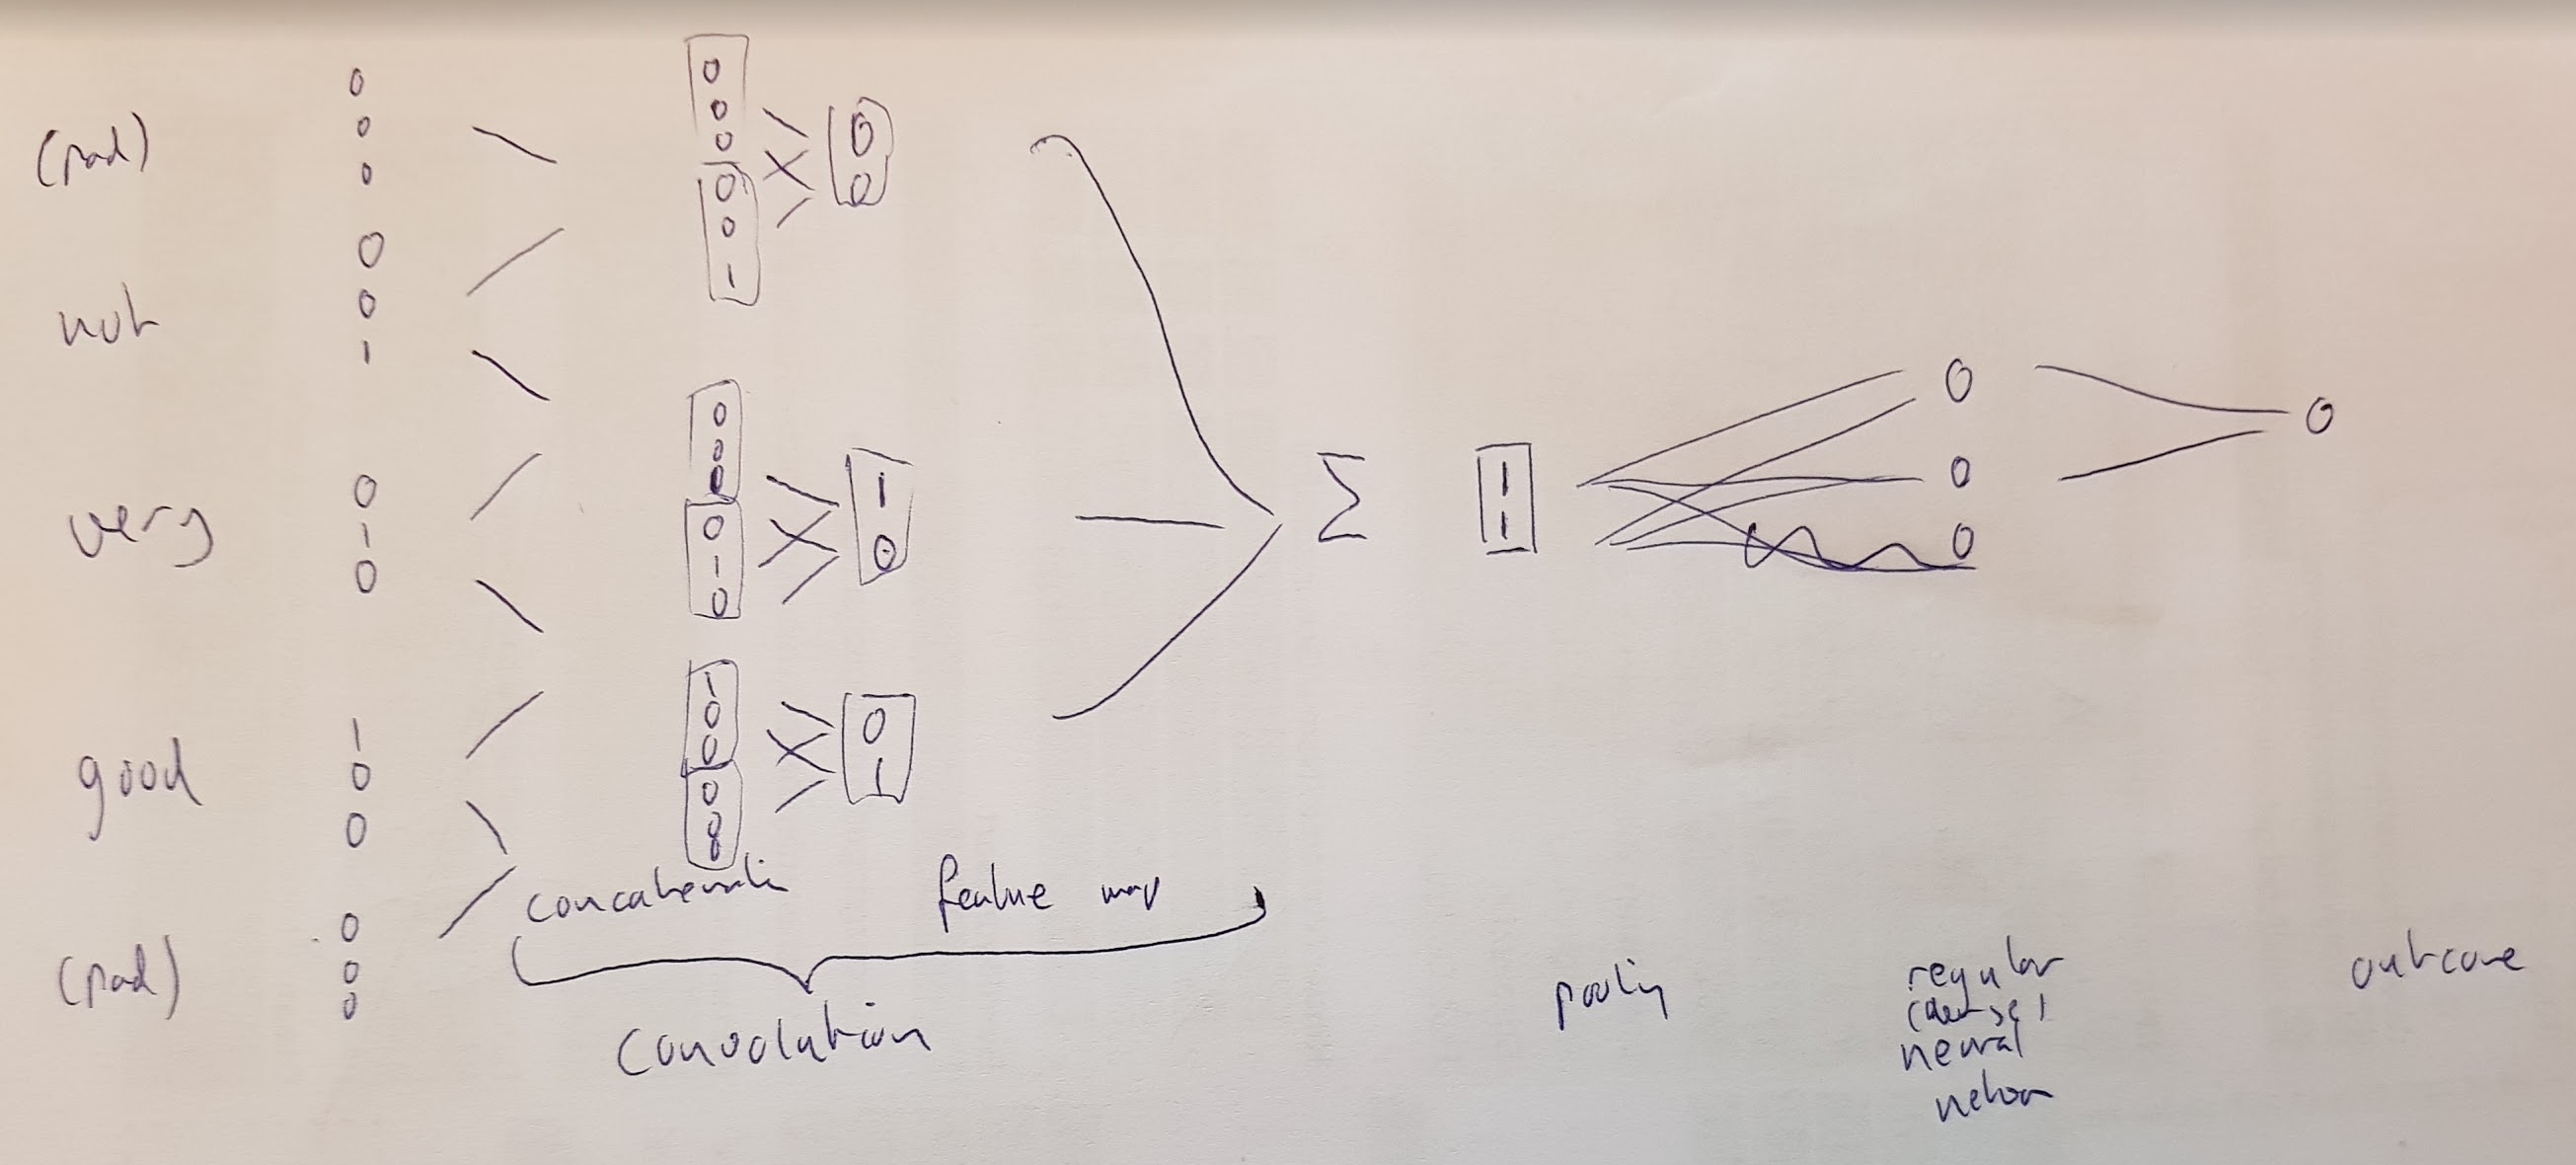
\includegraphics[width=\linewidth]{figures/ch09_cnn.png}
  \caption{Simplified example of a Convolutional Network applied to text analysis}
  \label{fig:cnn}
  \end{figure}

\reffig{cnn} shows a highly simplified example of this for text analysis of a sentence fragment `Would not recommend'.
The left hand shows how each word is encoded as a binary vector (e.g. 010 for `not', and 001 for `recommend').
In the second column, a shifting window concatenates these values for word pairs (so 010001 for `not recommend').
Next, a feature map layer detects interesting features in these concatenated values, for example
a feature for a negated positive term that has positive weights for negators in the first half and for positive words in the second.
These features are then pooled together to create document-level features,
for example by taking the maximum value per feature, which means that a feature is present in a document if it is present in any of the word windows in the document.
Finally, these document-level features are then used in a regular (dense) neural network which is connected to the output value, e.g. the document sentiment.
Since the convolutional layer is now connected with the output class, the feature maps can be automatically learned using the backpropagation algorithm explained above.
This means that the model can find the features in the word windows that are most helpful in predicting the document class, bringing the feature learning into the modelling process.

Of course, this is a highly simplified example, but it shows how local dependencies can be detected automatically using the convolutional network, as long as the interesting features are found within the specified word window.
Other architectures, such as the Long Short Term Memory mentioned above, can be used to also find non-local dependencies, but a full discussion of different architectures is well beyond the scope of this book.
\refchap{dtm} will give a more detailed example of deep learning for text analysis, where an embedding layer is combined with a convolutional network to build a sentiment analysis model. %TODO: CHECK AND CHANGE REFERENCE FOR TEXT ANALYSIS DEEP LEARNING MODEL.
Similarly, \refchap{image} will show how a similar technique can be used to extract features from small areas of images which are then used in automatic image classification.
This involves creating a two dimensional window over pixels rather than a unidimensional window over words, and often multiple convolutional layers are chained to detect features in increasingly large areas of the image.
The underlying technique of convolutional netoworks, however, is the same in both cases.


\section{Deep Learning}
\label{sec:deeplearning}

In Section~\ref{sec:neural}, we introduced neural networks with hidden layers and the backpropagation algorithm to fit them,
both of which date back to at least the 1970's.
In the past decade, however, the Artificial Intelligence community has been transformed by the introduction of  
\index{deep learning}\emph{deep learning},
where deep refers to a large amount of hidden layers between the input and output layers.
Many of the recent advances in AI, from self-driving cars to automatic translation and voice assistants,
are made possible by the application of deep learning techniques to the enormous amounts of digital data now becoming available.

An extensive treatment of deep learning is beyond the scope of this book (we recommend \cite{geron2019hands} instead).
However, in this section we will give you a brief introduction that should help you understand deep learning at a conceptual level,
and in Chapter~\ref{chap:dtm} and Chapter~\ref{chap:image} we will explain how these techniques can be applied to text analysis and visual analysis, respectively.

In principle, there is no clear demarcation between a ``classical'' neural network with hidden layers and a ``deep'' neural network.
There are three properties, however, that distinguish deep learning and explain why it is so successful: scale, structure, and feature learning.

\paragraph{Scale} First, and perhaps most importantly, deep learning models are many orders of magnitude larger and more complex than the models
trained in earlier decades.
This has been made possible by the confluence of unprecedented amounts of digital training data and increased computer processing power.
Partly, this has been enabled by the use of graphical processing units (GPUs), hardware designed for rendering the three-dimensional worlds used in games,
but that can also be used very efficiently for the computations needed to train neural networks (and mine bitcoins, but that's another story).

\paragraph{Structure} Most classical neural networks have only ``fully connected'' hidden layers with forward propagation,
meaning that each neuron in one layer is connected to each neuron in the next layer.
In deep learning, many specific architectures (some of which will be discussed below) are used to process information in certain ways,
limiting the number of parameters that need to be estimated.

\paragraph{Feature Learning}
In all models described so far with the exception of neural networks with hidden layers,
there was a direct relationship between the input features and the output class.
This meant that it is important to make sure that the required information the model needs to distinguish the classes
is directly encoded in the input features.
In the example used earlier, if ``not'' and ``good'' are separate features, a single-layer network (or a Na\"ive Bayes model)
cannot learn that these words together have a different meaning than the addition of their separate meanings.
However, similar to regression analysis, where you can create an interaction term or squared term to model a non-linear relationship,
the researcher can create input features for e.g.\ word pairs, for example including bigrams { (word pairs) such as ``not\_good''.
In fact, engineering the right features was the main way in which a researcher could improve model performance.
In deep learning, however, this feature learning step is generally included in the model itself,
with subsequent layers encoding different aspects of the raw data.

The properties of scale, structure, and feature learning are intertwined in deep learning: the much larger networks enable structures with beautiful names such as ``recurrent networks'', ``convolutional layers'' or ``long short-term memory'',
which are used to encode specific relationships and dependencies between features.
In this book, we will focus on convolutional networks as our only example of deep learning,
mostly because these networks are widely used in both text and image analysis.
Hopefully, this will give you insight into the general idea behind deep learning,
and you can learn about this and other models in more detail in the specialized resources cited above.

\subsection{Convolutional Neural Networks}
\label{sec:cnnbasis}

One challenge in many machine learning problems is a mismatch between the level of measurement of the output and the input.
For example, we normally want to  assign a single code such as sentiment or topic to a document or image.
The raw input, however, is at the word or pixel level.
In classical machine learning, this is generally solved by summarizing the input at the higher level of abstraction,
for example by using the total frequency of each word per document as input feature.
The problem is, however, that this summarization process removes a lot information that could be useful to the machine learning model,
for example combinations of words (``not good'') or their ordering (``John voted for Mary'' versus ``Mary voted for John''),
unless the researcher engineers features such as word pairs to add this information.

Convolutional Neural Networks are one way in which deep learning can overcome this limitation.
Essentially, the model internalizes the feature learning as a first part or ``layer'' of the model,
using a specialized network to summarize the raw input values into document (or image) level features.

% https://docs.google.com/drawings/d/1EySRM13hQoTcmEG1-J8b1Vz3CsNbW3aYsPt6J3ioD0o/edit
% pdfcrop -bbox "35 180 450 525" ch09_cnn.pdf ch09_cnn_cropped.pdf


\begin{figure}
  \centering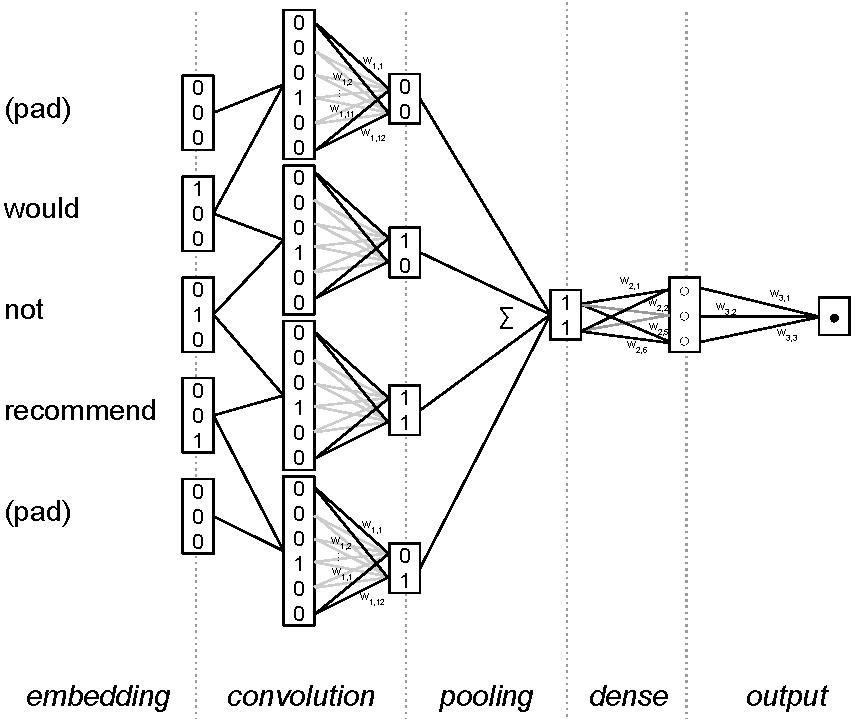
\includegraphics[width=.8\linewidth]{figures/ch09_cnn_cropped.pdf}
  \caption{Simplified example of a Convolutional Network applied to text analysis.}
  \label{fig:cnn}
  \end{figure}

Figure~\ref{fig:cnn} shows a highly simplified example of this for text analysis of a sentence fragment ``Would not recommend''.
The left hand side shows how each word is encoded as a binary vector (e.g.\ 010 for ``not'', and 001 for ``recommend'').
In the second column, a shifting window concatenates these values for word pairs (so 010001 for ``not recommend'').
Next, a feature map layer detects interesting features in these concatenated values, for example
a feature for a negated positive term that has positive weights for negators in the first half and for positive words in the second.
These features are then pooled together to create document-level features,
for example by taking the maximum value per feature, which means that a feature is present in a document if it is present in any of the word windows in the document.
Finally, these document-level features are then used in a regular (dense) neural network which is connected to the output value, e.g.\ the document sentiment.
Since the convolutional layer is now connected with the output class, the feature maps can be automatically learned using the backpropagation algorithm explained above.
This means that the model can find the features in the word windows that are most helpful in predicting the document class, bringing the feature learning into the modeling process.

Of course, this is a highly simplified example, but it shows how local dependencies can be detected automatically using the convolutional network, as long as the interesting features are found within the specified word window.
Other architectures, such as the Long Short Term Memory, can be used to also find non-local dependencies, but a full discussion of different architectures is well beyond the scope of this book.
Chapter~\ref{chap:dtm} will give a more detailed example of deep learning for text analysis, where an embedding layer is combined with a convolutional network to build a sentiment analysis model.
Similarly, Chapter~\ref{chap:image} will show how a similar technique can be used to extract features from small areas of images which are then used in automatic image classification.
This involves creating a two-dimensional window over pixels rather than a unidimensional window over words, and often multiple convolutional layers are chained to detect features in increasingly large areas of the image.
The underlying technique of convolutional networks, however, is the same in both cases.

%\section{Validation and best practices}
\label{sec:validation}
\subsection{Finding a balance between precision and recall}
\label{sec:balance}

In the previous sections, we have learned how to fit different models:
Na\"ive Bayes, logistic regressions, support vector machines, and
random forests.  We have also had a first look at confusion matrices,
precision, and recall.

But how do we find the best model? ``Best'', here, should be read as
``best for our purposes'' -- some models may be bad, and some may be
good, but which one is really the best may depend on what matters most
for us: Do we care more about precision or about recall? Are all
classes equally important to us?  And of course, other factors, such
as explainability or computational costs may factor into our decision.
 
But in any event, we need to decide which metrics to focus on.  We can
then either manually inspect them and look, for instance, which model
has the highest \emph{accuracy}, or the best balance of precision and recall,
or a recall higher than some threshold you are willing to accept.

If we build a classifier to distinguish spam messages from legitimate
messages, we could ask the following questions:
\begin{description}
\item[Precision] Which percentage of what our classifier predicts to be
  spam really is spam?
\item[Recall]{What percentage of all spam messages has our classifier
  found?}
\item[Accuracy]{In which percentage of all cases was our classifier
  right?}
\end{description}

We furthermore have:
\begin{description}
\item[F1-score]{The harmonic mean of precision and recall: $F_1 = 2
  \cdot \frac{precison \cdot recall}{precison + recall}$}
\item[AUC]{The AUC (Area under Curve) is the area under the curve that
  one gets when plotting the True Positive Rate (TPR) against the
  False Positive Rate (FPR) at various threshold settings. A perfect
  model will receive a value of 1.0, while random guessing between two
  equally probable classes will result in a value of 0.5}
\item[Micro- and macroaverage]{Especially when we have more than two
  classes, we can calculate the average of measures such as precision,
  recall, or f1-score. We can do so based on the separately calculated
  measures (macro), or based on the underlying values (TP, FP, etc.)
  (micro), which has different implications in the interpretation --
  especially if the classes have very different sizes.}
\end{description}


So, which one to choose?  If we really do not want to be annoyed by
any spam in our inbox, we need a high recall (we want to find all spam
messages). If, instead, we want to be sure that we do not
accidentally throw away legitimate messages, we need a high
precision (we want to be sure that all spam really is spam).

Maybe you say: well, I want both!  You could look at the accuracy, a
very straightforward to interpret measure. However, if you get many
more legitimate messages than spam (or the other way round), this
measure can be misleading: after all, even if your classifier finds
almost none of the spam messages (it has a recall close to zero), you
still get a very high accuracy, simply because there are so many
legitimate messages. In other words, the accuracy is not a good measure when working with highly unbalanced classes.
Often, it is therefore a better idea to look at the harmonic mean of
precision and recall, the F1-score, if you want to find a model that
gives you a good compromise between precision and recall.


In fact, we can even fine-tune our models in such a way that they are
geared towards either a better precision or a better recall.
As an example, let us take a logistic regression model. It predicts a
class label (such as ``spam'' versus ``legitimate''), but it can also
return the assigned probabilities. For a specific message, we can thus
say that we estimate its probability of being spam as, say, .65.
Unless we specify otherwise, everything above .5 will then be judged
to be spam, everything below as legitimate. But we could specify a
different cutoff point: we could, for instance, decide to classify
only everything above .7 as spam. This would give us a more
conservative spam filter, with probably a higher precision at the
expense of a lower recall.

\begin{figure} 
\centering
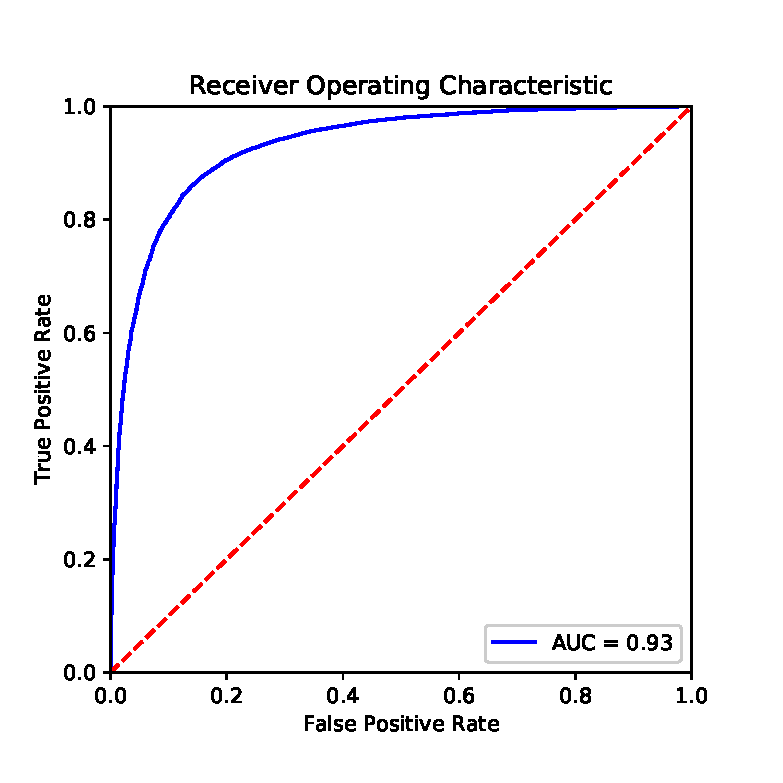
\includegraphics[width=0.4\linewidth]{figures/ch09_roccurve}
\caption{A ROC curve.}
\label{fig:roccurve}
\end{figure}

We can visualize this with a so-called ROC (reveicer operator
chraracteristic), a plot in which (Figure~\ref{fig:roccurve}) we plot
true positives against false positives at different thresholds.  A
good model extends until close to the upper left corner, and hence has
a large area under the curve (AUC).  If we choose a threshold at the
left end of the curve, we get few false positives (good!), but also
few true positives (bad!), if we go too far to the right, we get
the other extreme. So, how can we find the best spot?

One approach would be to print a table with three columns: the false
positive rate, the true positive rate, and the threshold value. You
then decide which FPR-TPR combination is most appealing to you, and
use the corresponding threshold value.

The second approach (also knwon as Yoden's J) is to find the threshold
value with the maximum distance between TPR and FPR, and use that one.

\pyrex[input=py, output=py,caption={Choosing a differnet cutoff point for predictions with logistic regression. In this case, we make a tradeoff and maximize the difference between false positive rate and true positive rate to improve the precision for the the second categegory by .12 at the expense of reducing the precision for the first category by .8.}]{chapter09/cutoffpoint}


\subsection{Train, validate, test}
\label{sec:train}

By now, we have established which measures we can use to decide which
model to use. For all of them, we have assumed that we split our
labeled dataset into two: a training dataset and a test dataset. The
logic behind it was simple: If we would calculate precision and recall
on the training data itself, our assessment would be too optimistic --
after all, our models have been trained on exactly these data, so
predicting the label isn't too hard. Assessing the models on a different
dataset, the test dataset, instead, gives us an assessment of how
precision and recall look like if haven't seen the labels earlier --
which is exactly what we want to know.

Unfortunately, if we calculate precision and recall (or any other
metric) for multiple models on the same test dataset, and use these
results to determine which metric to use, we can run into a problem:
We may avoid overfitting of our model on the training data, we may now
overfit it on the test data! After all, we could tweak our models as
long until they fit our test data perfectly, even if this makes the
predictions for other cases worse.

One way to avoid this is to split the original data into three
datasets instead of two: a training dataset, a validation dataset, and
a test dataset.  We train multiple model configurations on the
training dataset and calculate the metrics of interest for all of them
on the validation dataset.  Once we have decided on a final model, we
calculate its performance (once) on the test dataset, to get an
unbiased estimate of its performance.



\subsection{Cross-validation and grid search}
\label{sec:crossvalidation}
In an ideal world, we would have a huge labelled dataset and do not
need to worry about the decreasing size of our training dataset as we
set aside our validation and test datasets.

Unfortunately, our labelled datasets in the real world have a limited
size, and setting aside too many cases can be problematic. Especially
if you are already on a tight budget, setting aside not only a test
dataset, but also a validation dataset of meaningful size may lead to
critically small training datasets. While we have addressed the
problem of overfitting, this could lead to underfitting: We may have
removed the only examples of some specific feature combination, for
instance.

A common approach to address this issue is $k$-fold
cross-validation. To do so, we split our data into $k$ partitions,
so-called folds. We then estimate our model $k$ times, and each time
leave \emph{one} of the folds aside for validation. Hence, every fold
is exactly one time the validation dataset, and exactly $k-1$ times
part of the training data. We then simply average the results of our
$k$ values for the evaluation metric we are interested in.

If our classifier generalizes well, we would expect that our metric of
interest (e.g., the accuracy, or the f1-score, \ldots) is very similar
in all folds. ~\refex{crossval} performs a cross-validation based on
the logistic regression classifier we build above. We see that the
standard deviation is really low, indicating that there are almost no
changes between the runs, which is great.

Running the same cross-validation on our random forest, instead, would
produce not only worse (lower) means, but also worse (higher) standard
deviations, even though also here, there are no dramatic changes
between the runs.

\pyrex[input=both, output=both,caption=Crossvalidation]{chapter09/crossval}

Very often, cross-validation is used when we want to compare many
different model specifications, for example to find optimal
hyperparameters.
Hyperparameters are parameters of the model that are not estimated
from the data. These depend on the model, but could for example be the
estimation method to use, the number of times a bootstrap should be
repeated, etc. A very good example are the hyperparameters of support
vector machines (see above): It is hard to know how soft our margins
should be (the $C$), and we may also be unsure about the right kernel
(\refex{gridsearch2}), or in the case of a polinomial kernel, how many
degrees we want to consider.

Using the help function (e.g., \fn{RandomForestClassifier?} in Python),
you can look up
which hyperparameters you can specify. For a random forest classifier,
for instance, this includes the number of estimators in the model, the
criterion, and whether or not to use
bootstrapping. \refex{gridsearch}, \ref{ex:gridsearch2}, and
\ref{ex:gridsearch3} illustrate how you can automatically assess which
values you should choose.

\pyrex[input=py, output=py,caption=A simple gridsearch in Python]{chapter09/gridsearch}

\pyrex[input=py,output=py,caption=A gridsearch in Python using multiple CPUs]{chapter09/gridsearch2}

\pyrex[input=r,output=r,caption={A gridsearch in R. Note that in R, not all parameters are ``tunable'' using standard \pkg{caret}. Therefore, an exact replication of the grid searches in \refex{gridsearch} and \refex{gridsearch2} would requires either manual comparisons or writing a so-called caret extension.}]{chapter09/gridsearch3} 

\begin{feature}
    Supervised machine learning is one of the areas where you really
    see differences between Python and R. While in Python, virtually
    all you need is available via \pkg{scikit-learn}, in R, we often
    need to combine \pkg{caret} with various libraries providing the
    actual models. In contrast, all components we need for machine
    learning in Python are developed within one package, which leads
    to less friction. This is what you see in the gridsearch examples
    in this section. In scikit-learn, \emph{any} hyperparameter can be
    part of the grid, but no hyperparameter has to be.  Note that in
    R, in contrast, you cannot (at least, not easily) put any
    parameter of the model in the grid. Instead, you can look up the
    ``tunable parameters'' which \emph{must} be present part of the
    grid in the caret documentation. This means that an exact
    replication of the grid searches in \refex{gridsearch} and
    \refex{gridsearch2} is not natively supported using \pkg{caret}
    and requires either manual testing or writing a so-called caret
    extension.

    While in the end, you can find a supervised machine learning
    solution for all your use cases in R as well, if supervised
    machine learning is at the core of your project, it may save you a
    lot of cursing to do this in Python.
\end{feature}


\section{Validation and Best Practices}
\label{sec:validation}
\subsection{Finding a Balance Between Precision and Recall}
\label{sec:balance}

In the previous sections, we have learned how to fit different models:
Na\"ive Bayes, logistic regressions, support vector machines, and
random forests.  We have also had a first look at confusion matrices,
precision, and recall.

But how do we find the best model? ``Best'', here, should be read as
``best for our purposes'' -- some models may be bad, and some may be
good, but which one is really the best may depend on what matters most
for us: do we care more about precision or about recall? Are all
classes equally important to us?  And of course, other factors, such
as explainability or computational costs may factor into our decision.

But in any event, we need to decide which metrics to focus on.  We can
then either manually inspect them and look, for instance, which model
has the highest \emph{accuracy}, or the best balance of precision and recall,
or a recall higher than some threshold you are willing to accept.

If we build a classifier to distinguish spam messages from legitimate
messages, we could ask the following questions:
\begin{description}
\item[Precision] Which percentage of what our classifier predicts to be
  spam really is spam?
\item[Recall]{What percentage of all spam messages has our classifier
  found?}
\item[Accuracy]{In which percentage of all cases was our classifier
  right?}
\end{description}

We furthermore have:
\begin{description}
\item[$F_1$-score]{The harmonic mean of precision and recall: $F_1 = 2
  \cdot \frac{\rm precision \cdot recall}{\rm precision + recall}$}
\item[AUC]{The AUC (Area under Curve) is the area under the curve that
  one gets when plotting the True Positive Rate (TPR) against the
  False Positive Rate (FPR) at various threshold settings. A perfect
  model will receive a value of 1.0, while random guessing between two
  equally probable classes will result in a value of 0.5}
\item[Micro- and macro-average]{Especially when we have more than two
  classes, we can calculate the average of measures such as precision,
  recall, or  $F_1$-score. We can do so based on the separately calculated
  measures (macro), or based on the underlying values (TP, FP, etc.)
  (micro), which has different implications in the interpretation --
  especially if the classes have very different sizes.}
\end{description}


So, which one to choose?  If we really do not want to be annoyed by
any spam in our inbox, we need a high recall (we want to find all spam
messages). If, instead, we want to be sure that we do not
accidentally throw away legitimate messages, we need a high
precision (we want to be sure that all spam really is spam).

Maybe you say: well, I want both!  You could look at the accuracy, a
very straightforward to interpret measure. However, if you get many
more legitimate messages than spam (or the other way round), this
measure can be misleading: after all, even if your classifier finds
almost none of the spam messages (it has a recall close to zero), you
still get a very high accuracy, simply because there are so many
legitimate messages. In other words, the accuracy is not a good measure when working with highly unbalanced classes.
Often, it is therefore a better idea to look at the harmonic mean of
precision and recall, the $F_1$-score, if you want to find a model that
gives you a good compromise between precision and recall.


In fact, we can even fine-tune our models in such a way that they are
geared towards either a better precision or a better recall.
As an example, let us take a logistic regression model. It predicts a
class label (such as ``spam'' versus ``legitimate''), but it can also
return the assigned probabilities. For a specific message, we can thus
say that we estimate its probability of being spam as, say, 0.65.
Unless we specify otherwise, everything above 0.5 will then be judged
to be spam, everything below as legitimate. But we could specify a
different cutoff point: we could, for instance, decide to classify
 everything above 0.7 as spam. This would give us a more
conservative spam filter, with probably a higher precision at the
expense of a lower recall.

\begin{figure}
\centering
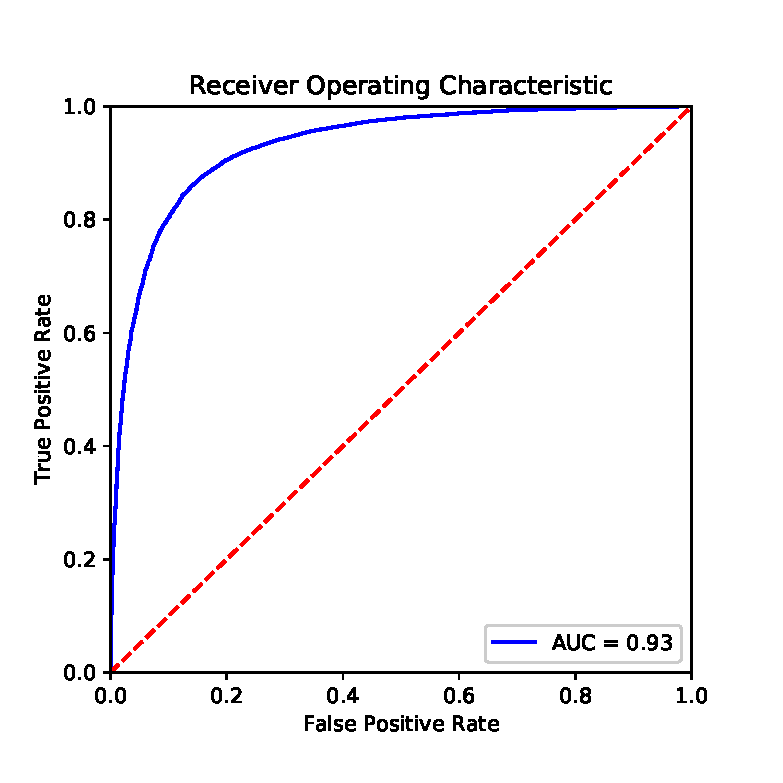
\includegraphics[width=0.4\linewidth]{figures/ch09_roccurve}
\caption{A (pretty good) ROC curve.}
\label{fig:roccurve}
\end{figure}

We can visualize this with a so-called ROC (receiver operator
characteristic), a plot in which (Figure~\ref{fig:roccurve}) we plot
true positives against false positives at different thresholds.  A
good model extends until close to the upper left corner, and hence has
a large area under the curve (AUC).  If we choose a threshold at the
left end of the curve, we get few false positives (good!), but also
few true positives (bad!), if we go too far to the right, we get
the other extreme. So, how can we find the best spot?

Example~\ref{ex:cutoffpoint} provides two approaches. One approach is to print a table with three columns: the false
positive rate, the true positive rate, and the threshold value. You
then decide which FPR--TPR combination is most appealing to you, and
use the corresponding threshold value. Having calculated the TPR and FPR anyway, we can
also additionally plot them as ROC curve (Example~\ref{ex:roccurve}), which may help
us interpreting the table.
The second approach (also knwon as Yoden's J) is to find the threshold
value with the maximum distance between TPR and FPR, and use that one.

\begin{ccsexample}
  \doublecodex{chapter08/cutoffpoint}
  \doubleoutput{chapter08/cutoffpoint}
  \doublecodex{chapter08/cutoffpointb}
  \doubleoutput{chapter08/cutoffpointb}
  Note: Python and R have slightly different outcomes because the underlying implementation is different, but for this example that may be ignored.
  \caption{Choosing a different cutoff point for predictions with logistic regression. In this case, we make a trade-off and maximize the difference between false positive rate and true positive rate to improve the precision for the the second category the precision for the first category}\label{ex:cutoffpoint}
\end{ccsexample}

\pyrex[output=py,format=png,caption={The ROC curve of a (not very impressive) classifier and its area under the curve (AUC)}]{chapter08/roccurve}



\subsection{Train, Validate, Test}
\label{sec:train}

By now, we have established which measures we can use to decide which
model to use. For all of them, we have assumed that we split our
labeled dataset into two: a training dataset and a test dataset. The
logic behind it was simple: if we  calculate precision and recall
on the training data itself, our assessment would be too optimistic --
after all, our models have been trained on exactly these data, so
predicting the label isn't too hard. Assessing the models on a different
dataset, the test dataset, instead, gives us an assessment of what
precision and recall look like if the labels  haven't been seen earlier --
which is exactly what we want to know.

Unfortunately, if we calculate precision and recall (or any other
metric) for multiple models on the same test dataset, and use these
results to determine which metric to use, we can run into a problem:
we may avoid overfitting of our model on the training data, we may now
overfit it on the test data! After all, we could tweak our models until they fit our test data perfectly, even if this makes the
predictions for other cases worse.

One way to avoid this is to split the original data into three
datasets instead of two: a training dataset, a validation dataset, and
a test dataset.  We train multiple model configurations on the
training dataset and calculate the metrics of interest for all of them
on the validation dataset.  Once we have decided on a final model, we
calculate its performance (once) on the test dataset, to get an
unbiased estimate of its performance.



\subsection{Cross-validation and Grid Search}
\label{sec:crossvalidation}
In an ideal world, we would have a huge labeled dataset and would not
need to worry about the decreasing size of our training dataset as we
set aside our validation and test datasets.

Unfortunately, our labeled datasets in the real world have a limited
size, and setting aside too many cases can be problematic. Especially
if you are already on a tight budget, setting aside not only a test
dataset, but also a validation dataset of meaningful size may lead to
critically small training datasets. While we have addressed the
problem of overfitting, this could lead to underfitting: we may have
removed the only examples of some specific feature combination, for
instance.

A common approach to address this issue is $k$-fold
cross-validation. To do this, we split our data into $k$ partitions,
so-called folds. We then estimate our model $k$ times, and each time
leave \emph{one} of the folds aside for validation. Hence, every fold
is exactly one time the validation dataset, and exactly $k-1$ times
part of the training data. We then simply average the results of our
$k$ values for the evaluation metric we are interested in.

If our classifier generalizes well, we would expect that our metric of
interest (e.g., the accuracy, or the $F_1$-score, \ldots) is very similar
in all folds. ~Example~\ref{ex:crossval} performs a cross-validation based on
the logistic regression classifier we built above. We see that the
standard deviation is really low, indicating that there are almost no
changes between the runs, which is great.

Running the same cross-validation on our random forest, instead, would
produce not only worse (lower) means, but also worse (higher) standard
deviations, even though also here, there are no dramatic changes
between the runs.

\pyrex[input=both, output=both,caption=Crossvalidation]{chapter08/crossval}

Very often, cross-validation is used when we want to compare many
different model specifications, for example to find optimal
hyperparameters.
Hyperparameters are parameters of the model that are not estimated
from the data. These depend on the model, but could for example be the
estimation method to use, the number of times a bootstrap should be
repeated, etc. Very good examples are the hyperparameters of support
vector machines (see above): it is hard to know how soft our margins
should be (the $C$), and we may also be unsure about the right kernel
(Example~\ref{ex:gridsearch2}), or in the case of a polinomial kernel, how many
degrees we want to consider.

Using the help function (e.g., \index{RandomForestClassifier?}\texttt{RandomForestClassifier?} in Python),
you can look up
which hyperparameters you can specify. For a random forest classifier,
for instance, this includes the number of estimators in the model, the
criterion, and whether or not to use
bootstrapping. Example~\ref{ex:gridsearch}, \ref{ex:gridsearch2}, and
\ref{ex:gridsearch3} illustrate how you can automatically assess which
values you should choose.

\pyrex[input=py, output=py,caption=A simple gridsearch in Python]{chapter08/gridsearch}

\pyrex[input=py,output=py,caption=A gridsearch in Python using multiple CPUs]{chapter08/gridsearch2}

\pyrex[input=r,output=r,caption={A gridsearch in R. Note that in R, not all parameters are ``tunable'' using standard \index{caret}\emph{caret}. Therefore, an exact replication of the grid searches in Example~\ref{ex:gridsearch} and Example~\ref{ex:gridsearch2} would requires either manual comparisons or writing a so-called caret extension.}]{chapter08/gridsearch3}

\begin{feature}
    Supervised machine learning is one of the areas where you really
    see differences between Python and R. While in Python, virtually
    all you need is available via \index{scikit-learn}\emph{scikit-learn}, in R, we often
    need to combine \index{caret}\emph{caret} with various libraries providing the
    actual models. In contrast, all components we need for machine
    learning in Python are developed within one package, which leads
    to less friction. This is what you see in the gridsearch examples
    in this section. In scikit-learn, \emph{any} hyperparameter can be
    part of the grid, but no hyperparameter has to be.  Note that in
    R, in contrast, you cannot (at least, not easily) put any
    parameter of the model in the grid. Instead, you can look up the
    ``tunable parameters'' which \emph{must} be present as part of the
    grid in the caret documentation. This means that an exact
    replication of the grid searches in Example~\ref{ex:gridsearch} and
    Example~\ref{ex:gridsearch2} is not natively supported using \index{caret}\emph{caret}
    and requires either manual testing or writing a so-called caret
    extension.

    While in the end, you can find a supervised machine learning
    solution for all your use cases in R as well, if supervised
    machine learning is at the core of your project, it may save you a
    lot of cursing to do this in Python.
\end{feature}
